\documentclass[Skript.tex]{subfiles} 
\begin{document}


\section{Aufbau}


\subsection{Spielbeschreibung}

\gname ist ein Platformer, bei dem über eine eingelesene Musikdatei die Karte generiert wird.
Der Spieler muss Genre-typischen Hindernissen ausweichen (hüpfen, ducken usw.).

Der Designschwerpunkt des Spiels liegt in der Idee, dass der Spieler eine gewünschte Musikdatei einlesen kann und die daraus generierte Karte im Anschluss spielt. 
Während der Spieler sich durch das Level bewegt und hin und wieder Punkte einsammelt, wird passend dazu seine vorher eingelesene Musik abgespielt.

Das Grundgameplay besteht aus dem Ziel, Hindernissen solange auszuweichen bis das Lied vorbei ist, und dabei so viele Punkte wie möglich zu sammeln.


\subsection{Visuelle Präsentation}

\begin{wrapfigure}[9]{r}{4cm}
\vspace{-1.2cm}
  \begin{center}
    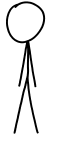
\includegraphics[scale=.9]{Grafik/char.png}
	\caption{Standard Charakter}
	\label{charakter}
  \end{center}
\end{wrapfigure}

Der Stil des Spiels \gname lehnt sich an die Comics von \textit{Randall Munroe} an.
Hier dienen die Charaktere von \href{http://xkcd.com}{xkcd.com} als Vorlage.

Die Lizenz \href{http://creativecommons.org/licenses/by-nc/2.5/}{creativecommons.org} erlaubt uns, Material mitzubenutzen und zu verändern.
Voraussetzung dafür, ist darauf zu verweisen (Webseite, Lizenz) und keinen kommerziellen Nutzen daraus zu ziehen.


Der Spieler spielt einen gesichtslosen Charakter (Strichmännchen). 
Die Umgebung, in der sich der Charakter bewegt, vermittelt den Eindruck einer Schreibtischunterlage. 
Das Spiel sieht aus wie handgemalt, allerdings werden die Sterbe-Animation mit viel Blut dargestellt.




\subsection{Featureliste}

\begin{itemize}
\item Musikdatei einlesen (im Optionen-Menü)
\item Springen (Leertaste)
\item Ducken  (Pfeil nach unten)
\item Gleiten (Leertaste gedrückt halten)
\item Teleport (Pfeil nach oben)
\end{itemize}


\subsection{Spielbestandteile}

Der Spieler läuft  in \gname mit dem Strichmännchen durch die selbstgenerierte Karte und muss während des Levels Hindernissen ausweichen. Diese sind z.\,B.\ :

\begin{itemize}
\item Plattform auf die man Springen bzw.\ unter der Plattform durchlaufen kann: Radiergummi, Taschenrechner
\item Plattform auf die man Springen muss: Post-It
\item Stachelhaufen: Reißzwecken
\item Schluchten (zwei Größen)
\end{itemize}

Es gibt Schluchten, die zu groß sind um sie zu überspringen. 
Deshalb muss der Spieler den Gleiten-Modus nutzen, um nicht zu verlieren. 
Dieser Modus verbraucht eine spezielle Resource (Füllstandsanzeige in der GUI).
Diese lädt sich nur auf, wenn der Spieler läuft oder geduckt läuft.

Das Ziel wird erreicht, indem der Spieler solange den Hindernissen ausweicht bis das Lied zu Ende ist.
Wenn das Ausweichen eines Hindernisses misslingt, verliert der Charakter eines seiner anfangs drei Leben, bzw.\ stirbt, wenn diese aufgebraucht sind (Loosecondition).  


\subsection{Rewards}

Rewards werden in drei Kategorien eingeteilt: Klein, Mittel und Groß.

\begin{description}
\item[Kleine Rewards: ]	%TODO ZEILENUMBRUCH
Der Spieler wird belohnt indem er Punkte einsammelt. 
Dies kann alle paar Sekunden geschehen indem er an entsprechenden Stellen springt.

\item[Mittlere Rewards: ] Der Spieler schafft ein Level.
Er wird mit einer Zielanimation und seinem erreichten Punktestand belohnt.

\item[Großer Reward: ] Der Spieler bekommt nach dem ersten geschafften Level einen neuen Skin zur Verfügung.
Weitere Skins werden nach fünf und nach zehn Siegen freigeschaltet.
\end{description}


\subsection{Technologie}

\begin{itemize}
\item Minim (Soundbibliothek für Processing) zur Soundanalyse
\item XNA Spieleentwicklung
\end{itemize}

\subsubsection{Used Software}

\begin{itemize}
\item Dokumentation:  Miktex (\LaTeX)
\item Programmierung:  MS VisualStudio 2010
\item Programmierung:  Processing 2.08b
\end{itemize}


\subsection{Entwicklungszeitrahmen}
Für das Projekt stenden zwei Wochen Entwicklungszeit zur Verfügung.


\subsection{Unique Features}

\begin{itemize}
\item Eine Karte die aus Audiodateien individuell generiert wird.
\item Einsammelbare Boni werden anhand der Beat-Erkennung platziert.
\item Cheat-Modus, der den Spieler über das Level schweben lässt.
\end{itemize}


\subsection{Gameplay-Beispiel}

Der Spieler startet das Spiel.
Im Optionen-Menü wählt er seine individuelle Musikdatei aus und generiert damit das Level. 
Anschließend verlässt er das Optionen-Menü und startet das Level.
Der Charakter bewegt sich mit konstantem Tempo nach rechts.
Nach einer kleinen Aufwärmphase erscheint das erste Hindernis.
Der Spieler muss entsprechend dem Hindernis reagieren und die richtige Taste drücken um diesem auszuweichen.
Erscheint hier eine Plattform in Form eines Post-Its auf dem Boden, springt der Spieler durch das rechtzeitige Drücken der Leertaste hoch, landet auf dem Hindernis und läuft weiter.
Als Alternatives Hindernis erscheint ein Radiergummi, der in der Luft schwebt.
Hier kann der Spieler entscheiden, ob er darauf springt oder unter dem Hindernis hindurch duckt.
Bestimmte Hindernisse wie kurze Schluchten und Reißzweckenhaufen müssen ebenfalls übersprungen werden.
Lange Schluchten allerdings können nicht übersprungen werden, sondern müssen mittels Gleitsprung (gehaltene Leertaste) überwunden werden.
Falls die Ressource für den Gleitsprung leer ist, fällt der Spieler herunter.\\

Stirbt der Spieler, verlassen die bereits eingesammelten Noten (= Punkte) den Körper und zerplatzen.\\

Am Anfang jedes Levels kann man einen QR-Code entdecken.
Dieser enthält einen Hinweis auf die Cheat-Aktivierung.
Im Cheat-Modus schwebt der Spieler in einer anderen Dimension über das Level und sammelt automatisch alle Boni ein.
Allerdings zählt ein durch Cheat errungener Sieg nicht für die Freischaltung der anderen Skins.





\end{document}